% 若编译失败,且生成 .synctex(busy) 辅助文件,可能有两个原因:
% 1. 需要插入的图片不存在:Ctrl + F 搜索 'figure' 将这些代码注释/删除掉即可
% 2. 路径/文件名含中文或空格:更改路径/文件名即可

% --------------------- 文章宏包及相关设置 --------------------- %
% >> ------------------ 文章宏包及相关设置 ------------------ << %
% 设定文章类型与编码格式
\documentclass[UTF8]{article}		

% 本文所需的特殊宏包

% 本 .tex 专属的宏定义
    \def\V{\ \mathrm{V}}
    \def\uV{\ \mu\mathrm{V}}
    \def\mV{\ \mathrm{mV}}
    \def\K{\ \mathrm{K}}
    \def\kV{\ \mathrm{KV}}
    \def\KV{\ \mathrm{KV}}
    \def\MV{\ \mathrm{MV}}
    \def\uA{\ \mu\mathrm{A}}
    \def\mA{\ \mathrm{mA}}
    \def\A{\ \mathrm{A}}
    \def\kA{\ \mathrm{KA}}
    \def\KA{\ \mathrm{KA}}
    \def\MA{\ \mathrm{MA}}
    \def\O{\ \Omega}
    \def\mO{\ \Omega}
    \def\kO{\ \mathrm{K}\Omega}
    \def\KO{\ \mathrm{K}\Omega}
    \def\MO{\ \mathrm{M}\Omega}
    \def\Hz{\ \mathrm{Hz}}
    \def\uF{\ \mu\mathrm{F}}
    \def\mF{\ \mathrm{mF}}
    \def\nF{\ \mathrm{nF}}
    \def\F{\ \mathrm{F}}
    \def\Re{\mathrm{\,Re}\,}
    \def\Im{\mathrm{\,Im}\,}
    \def\sinc{\mathrm{\,sinc}\,}

% 自定义宏定义
    \def\N{\mathbb{N}}
    \def\F{\mathbb{F}}
    \def\Z{\mathbb{Z}}
    \def\Q{\mathbb{Q}}
    \def\R{\mathbb{R}}
    \def\C{\mathbb{C}}
    \def\T{\mathbb{T}}
    \def\S{\mathbb{S}}
    %\def\A{\mathbb{A}}
    \def\I{\mathscr{I}}
    \def\d{\mathrm{d}}
    \def\p{\partial}

    
% 本 .tex 专属的宏定义
\def\V{\ \mathrm{V}}
\def\uV{\ \mu\mathrm{V}}
\def\mV{\ \mathrm{mV}}
\def\K{\ \mathrm{K}}
\def\kV{\ \mathrm{KV}}
\def\KV{\ \mathrm{KV}}
\def\MV{\ \mathrm{MV}}
\def\uA{\ \mu\mathrm{A}}
\def\mA{\ \mathrm{mA}}
\def\A{\ \mathrm{A}}
\def\kA{\ \mathrm{KA}}
\def\KA{\ \mathrm{KA}}
\def\MA{\ \mathrm{MA}}
\def\O{\ \Omega}
\def\mO{\ \Omega}
\def\kO{\ \mathrm{K}\Omega}
\def\KO{\ \mathrm{K}\Omega}
\def\MO{\ \mathrm{M}\Omega}
\def\Hz{\ \mathrm{Hz}}
\def\uF{\ \mu\mathrm{F}}
\def\mF{\ \mathrm{mF}}
\def\F{\ \mathrm{F}}

% 自定义宏定义
\def\N{\mathbb{N}}
%\def\F{\mathbb{F}}
\def\Z{\mathbb{Z}}
\def\Q{\mathbb{Q}}
\def\R{\mathbb{R}}
\def\C{\mathbb{C}}
\def\T{\mathbb{T}}
\def\S{\mathbb{S}}
\def\A{\mathbb{A}}
\def\I{\mathscr{I}}
\def\Im{\mathrm{Im\,}}
\def\Re{\mathrm{Re\,}}
\def\d{\mathrm{d}}
\def\p{\partial}


% 导入基本宏包
    \usepackage[UTF8]{ctex}     % 设置文档为中文语言
    \usepackage{hyperref}  % 宏包:自动生成超链接 (此宏包与标题中的数学环境冲突)
    \hypersetup{
        colorlinks=true,    % false:边框链接 ; true:彩色链接
        citecolor={blue},    % 文献引用颜色
        linkcolor={blue},   % 目录 (我们在目录处单独设置),公式,图表,脚注等内部链接颜色
        urlcolor={magenta},    % 网页 URL 链接颜色,包括 \href 中的 text
        % cyan 浅蓝色 
        % magenta 洋红色
        % yellow 黄色
        % black 黑色
        % white 白色
        % red 红色
        % green 绿色
        % blue 蓝色
        % gray 灰色
        % darkgray 深灰色
        % lightgray 浅灰色
        % brown 棕色
        % lime 石灰色
        % olive 橄榄色
        % orange 橙色
        % pink 粉红色
        % purple 紫色
        % teal 蓝绿色
        % violet 紫罗兰色
    }
    % \usepackage{docmute}    % 宏包:子文件导入时自动去除导言区,用于主/子文件的写作方式,\include{./51单片机笔记}即可。注:启用此宏包会导致.tex文件capacity受限。
    \usepackage{amsmath}    % 宏包:数学公式
    \usepackage{mathrsfs}   % 宏包:提供更多数学符号
    \usepackage{amssymb}    % 宏包:提供更多数学符号
    \usepackage{pifont}     % 宏包:提供了特殊符号和字体
    \usepackage{extarrows}  % 宏包:更多箭头符号 
    \usepackage{multicol}   % 宏包:支持多栏 

% 文章页面margin设置
    \usepackage[a4paper]{geometry}
        \geometry{top=0.75in}
        \geometry{bottom=0.75in}
        \geometry{left=0.75in}
        \geometry{right=0.75in}   % 设置上下左右页边距
        \geometry{marginparwidth=1.75cm}    % 设置边注距离(注释、标记等)

% 配置数学环境
    \usepackage{amsthm} % 宏包:数学环境配置
    % theorem-line 环境自定义
        \newtheoremstyle{MyLineTheoremStyle}% <name>
            {11pt}% <space above>
            {11pt}% <space below>
            {\kaishu}% <body font> 默认使用正文字体, \kaishu 为楷体
            {}% <indent amount>
            {\bfseries}% <theorem head font> 设置标题项为加粗
            {:\ \ }% <punctuation after theorem head>
            {.5em}% <space after theorem head>
            {\textbf{#1}\thmnumber{#2}\ \ (\,\textbf{#3}\,)}% 设置标题内容顺序
        \theoremstyle{MyLineTheoremStyle} % 应用自定义的定理样式
        \newtheorem{LineTheorem}{Theorem.\,}
    % theorem-block 环境自定义
        \newtheoremstyle{MyBlockTheoremStyle}% <name>
            {11pt}% <space above>
            {11pt}% <space below>
            {\kaishu}% <body font> 使用默认正文字体
            {}% <indent amount>
            {\bfseries}% <theorem head font> 设置标题项为加粗
            {:\\ \indent}% <punctuation after theorem head>
            {.5em}% <space after theorem head>
            {\textbf{#1}\thmnumber{#2}\ \ (\,\textbf{#3}\,)}% 设置标题内容顺序
        \theoremstyle{MyBlockTheoremStyle} % 应用自定义的定理样式
        \newtheorem{BlockTheorem}[LineTheorem]{Theorem.\,} % 使用 LineTheorem 的计数器
    % definition 环境自定义
        \newtheoremstyle{MySubsubsectionStyle}% <name>
            {11pt}% <space above>
            {11pt}% <space below>
            {}% <body font> 使用默认正文字体
            {}% <indent amount>
            {\bfseries}% <theorem head font> 设置标题项为加粗
            {:\\ \indent}% <punctuation after theorem head>
            {0pt}% <space after theorem head>
            {\textbf{#3}}% 设置标题内容顺序
        \theoremstyle{MySubsubsectionStyle} % 应用自定义的定理样式
        \newtheorem{definition}{}

%宏包:有色文本框(proof环境)及其设置
    \usepackage{xcolor}    %设置插入的文本框颜色
    \usepackage[strict]{changepage}     % 提供一个 adjustwidth 环境
    \usepackage{framed}     % 实现方框效果
        \definecolor{graybox_color}{rgb}{0.95,0.95,0.96} % 文本框颜色。修改此行中的 rgb 数值即可改变方框纹颜色,具体颜色的rgb数值可以在网站https://colordrop.io/ 中获得。(截止目前的尝试还没有成功过,感觉单位不一样)(找到喜欢的颜色,点击下方的小眼睛,找到rgb值,复制修改即可)
        \newenvironment{graybox}{%
        \def\FrameCommand{%
        \hspace{1pt}%
        {\color{gray}\vrule width 2pt}%
        {\color{graybox_color}\vrule width 4pt}%
        \colorbox{graybox_color}%
        }%
        \MakeFramed{\advance\hsize-\width\FrameRestore}%
        \noindent\hspace{-4.55pt}% disable indenting first paragraph
        \begin{adjustwidth}{}{7pt}%
        \vspace{2pt}\vspace{2pt}%
        }
        {%
        \vspace{2pt}\end{adjustwidth}\endMakeFramed%
        }

% 外源代码插入设置
    % matlab 代码插入设置
    \usepackage{matlab-prettifier}
        \lstset{style=Matlab-editor}    % 继承 matlab 代码高亮 , 此行不能删去
    \usepackage[most]{tcolorbox} % 引入tcolorbox包 
    \usepackage{listings} % 引入listings包
        \tcbuselibrary{listings, skins, breakable}
        \newfontfamily\codefont{Consolas} % 定义需要的 codefont 字体
        \lstdefinestyle{MatlabStyle_inc}{   % 插入代码的样式
            language=Matlab,
            basicstyle=\footnotesize\ttfamily\codefont,    % ttfamily 确保等宽 
            breakatwhitespace=false,
            breaklines=true,
            captionpos=b,
            keepspaces=true,
            numbers=left,
            numbersep=15pt,
            showspaces=false,
            showstringspaces=false,
            showtabs=false,
            tabsize=2,
            xleftmargin=15pt,   % 左边距
            %frame=single, % single 为包围式单线框
            frame=shadowbox,    % shadowbox 为带阴影包围式单线框效果
            %escapeinside=``,   % 允许在代码块中使用 LaTeX 命令 (此行无用)
            %frameround=tttt,    % tttt 表示四个角都是圆角
            framextopmargin=0pt,    % 边框上边距
            framexbottommargin=0pt, % 边框下边距
            framexleftmargin=5pt,   % 边框左边距
            framexrightmargin=5pt,  % 边框右边距
            rulesepcolor=\color{red!20!green!20!blue!20}, % 阴影框颜色设置
            %backgroundcolor=\color{blue!10}, % 背景颜色
        }
        \lstdefinestyle{MatlabStyle_src}{   % 插入代码的样式
            language=Matlab,
            basicstyle=\small\ttfamily\codefont,    % ttfamily 确保等宽 
            breakatwhitespace=false,
            breaklines=true,
            captionpos=b,
            keepspaces=true,
            numbers=left,
            numbersep=15pt,
            showspaces=false,
            showstringspaces=false,
            showtabs=false,
            tabsize=2,
        }
        \newtcblisting{matlablisting}{
            %arc=2pt,        % 圆角半径
            % 调整代码在 listing 中的位置以和引入文件时的格式相同
            top=0pt,
            bottom=0pt,
            left=-5pt,
            right=-5pt,
            listing only,   % 此句不能删去
            listing style=MatlabStyle_src,
            breakable,
            colback=white,   % 选一个合适的颜色
            colframe=black!0,   % 感叹号后跟不透明度 (为 0 时完全透明)
        }
        \lstset{
            style=MatlabStyle_inc,
        }

% table 支持
    \usepackage{booktabs}   % 宏包:三线表
    \usepackage{tabularray} % 宏包:表格排版
    \usepackage{longtable}  % 宏包:长表格

% figure 设置
    \usepackage{graphicx}  % 支持 jpg, png, eps, pdf 图片 
    \usepackage{svg}       % 支持 svg 图片
        \svgsetup{
            % 指向 inkscape.exe 的路径
            inkscapeexe = C:/aa_MySame/inkscape/bin/inkscape.exe, 
            % 一定程度上修复导入后图片文字溢出几何图形的问题
            inkscapelatex = false                 
        }
    \usepackage{subcaption} % 用于子图和小图注  

% 图表进阶设置
    \usepackage{caption}    % 图注、表注
        \captionsetup[figure]{name=图}  
        \captionsetup[table]{name=表}
        \captionsetup{
            labelfont=bf, % 设置标签为粗体
            textfont=bf,  % 设置文本为粗体
            font=small  
        }
    \usepackage{float}     % 图表位置浮动设置 
    \usepackage{etoolbox} % 用于保证图注表注的数学字符为粗体
        \AtBeginEnvironment{figure}{\boldmath} % 图注中的数学字符为粗体
        \AtBeginEnvironment{table}{\boldmath}  % 表注中的数学字符为粗体
        \AtBeginEnvironment{tabular}{\unboldmath}   % 保证表格中的数学字符不受额外影响

% 圆圈序号自定义
    \newcommand*\circled[1]{\tikz[baseline=(char.base)]{\node[shape=circle,draw,inner sep=0.8pt, line width = 0.03em] (char) {\bfseries #1};}}   % TikZ solution

% 列表设置
    \usepackage{enumitem}   % 宏包:列表环境设置
        \setlist[enumerate]{
            label=(\arabic*) ,   % 设置序号样式为加粗的 (1) (2) (3)
            ref=\arabic*, % 如果需要引用列表项,这将决定引用格式(这里仍然使用数字)
            itemsep=0pt, parsep=0pt, topsep=0pt, partopsep=0pt, leftmargin=3.5em} 
        \setlist[itemize]{itemsep=0pt, parsep=0pt, topsep=0pt, partopsep=0pt, leftmargin=3.5em}
        \newlist{circledenum}{enumerate}{1} % 创建一个新的枚举环境  
        \setlist[circledenum,1]{  
            label=\protect\circled{\arabic*}, % 使用 \arabic* 来获取当前枚举计数器的值,并用 \circled 包装它  
            ref=\arabic*, % 如果需要引用列表项,这将决定引用格式(这里仍然使用数字)
            itemsep=0pt, parsep=0pt, topsep=0pt, partopsep=0pt, leftmargin=3.5em
        }  

% 其它设置
    % 脚注设置
        \renewcommand\thefootnote{\ding{\numexpr171+\value{footnote}}}
    % 参考文献引用设置
        \bibliographystyle{unsrt}   % 设置参考文献引用格式为unsrt
        %\bibliographystyle{ieeetr}   % 设置参考文献引用格式为unsrt
        \newcommand{\upcite}[1]{\textsuperscript{\cite{#1}}}     % 自定义上角标式引用
    % 文章序言设置
        \newcommand{\cnabstractname}{序言}
        \newenvironment{cnabstract}{%
            \par\Large
            \noindent\mbox{}\hfill{\bfseries \cnabstractname}\hfill\mbox{}\par
            \vskip 2.5ex
            }{\par\vskip 2.5ex}

% 文章默认字体设置
    \usepackage{fontspec}   % 宏包:字体设置
        \setmainfont{SimSun}    % 设置中文字体为宋体字体
        \setCJKmainfont[AutoFakeBold=3]{SimSun} % 设置加粗字体为 SimSun 族,AutoFakeBold 可以调整字体粗细
        \setmainfont{Times New Roman} % 设置英文字体为Times New Roman

% 各级标题自定义设置
    \usepackage{titlesec}   
        % section标题自定义设置 
        \titleformat{\section}[hang]{\normalfont\Large\bfseries\boldmath}{\thesection}{8pt}{}
        % subsection 标题自定义设置
        \titleformat{\subsection}[hang]{\normalfont\large\bfseries\boldmath}{\thesubsection}{8pt}{}
        \titlespacing*{\subsection}{0pt}{10pt}{6pt} % 控制上下间距


% --------------------- 文章宏包及相关设置 --------------------- %
% >> ------------------ 文章宏包及相关设置 ------------------ << %


% ------------------------ 文章信息区 ------------------------ %
% ------------------------ 文章信息区 ------------------------ %
% 页眉页脚设置
\usepackage{fancyhdr}   %宏包:页眉页脚设置
\usepackage{fontawesome}    % 宏包:更多符号与图标 (用于插入 GitHub 图标等)
    \pagestyle{fancy}
    \fancyhf{}
    \cfoot{\thepage}
    \renewcommand\headrulewidth{1pt}
    \renewcommand\footrulewidth{0pt}
    \chead{Buck Circuit Design, 丁毅}
    \lhead{
    \href{https://github.com/YiDingg/LatexNotes}{\color{black}\faGithub\ https://github.com/YiDingg/LatexNotes}
    }
    \rhead{dingyi233@mails.ucas.ac.cn}

% 开始编辑文章

\begin{document}
\setcounter{page}{81}

\begin{center}\large
    \vspace*{-0.8cm}
    \noindent{\huge\bfseries An \ \ Improved \ \ Buck \ \ Circuit}\\\vspace{0.2cm}
    \noindent{\Large\bfseries 《\ 电\ 路\ 原\ 理》\ 电\ 路\ 设\ 计\ 报\ 告 }\\
    \noindent{\large\bfseries 2024.11.07 - 2024.12.31}
\end{center}
\vspace{-0.5cm}
\noindent\rule{\textwidth}{0.075em}   % 分割线
\vspace{-1.0cm}

% 目录
\setcounter{tocdepth}{2}  % 目录深度为 2(不显示 subsubsection)
\noindent\tableofcontents\thispagestyle{fancy}   % 显示页码、页眉等
\newpage
% ------------------------ 文章信息区 ------------------------ %
% ------------------------ 文章信息区 ------------------------ %


%% 下面是正文内容

Buck 电路是一种开关型 DC-DC 变换器,用于将输入的(高)直流电压转换为输出(低)直流电压。在本次,我们将设计一个开关频率和占空比可调的 Buck 电路。其中,开关频率主要影响输出的正弦(三角)纹波大小,占空比可以控制输出电压大小。

需要注意的是,开关频率和占空比都可能影响电路的稳定性(如抗噪性能),实际使用时应做抗干扰测试,或者进一步改进后再使用。


\section{设计要求}
利用运算放大器 OPA 和 MOSFET 实现 Buck 电路,下面是具体的设计要求:
\begin{enumerate}
\item 输出电压 3.3 V,电压输出纹波比 $r = \frac{\Delta U_{\text{o}}}{U_{\text{o, ave}}} < 5\%$,$3.3\ \mathrm{V}\times 5\,\% = 165\ \mathrm{mV}$,相当于 $\pm\, 82.2\ \mathrm{mV}$;
\item 使用一个 +15 V 电源和一个 -15 V 电源供电;
\item MOSFET 型号为 2N7000;
\item 运放型号为 LM258N;
\item 整流二极管型号为 1N4007;
\item 电阻电容电感数量不限;最后的滤波电容最大值不超过 470 $\uF$,最后的负载电阻不要小于 2 $\kO$;
\item 电感非理想,所以需要测试电感的 Q 值和 DCR (Direct Current Resistance),仿真时将 DCR 考虑进去;
\item 电容非理想,所以需要测试电容的 ESR (Equivalent Series Resistance) 和实际容值;
\item 实验报告里面包含原理说明、设计的电路图、仿真结果、实际电路照片、实际电路测试结果及分析。
\end{enumerate}


\section{脉冲发生器}

\subsection{脉冲发生器原理}
Buck 电路中最关键的无疑是 MOS 的开关作用,为了能产生提供给 MOSFET 的脉冲电压,我们先讨论脉冲发生器 (Pulse Generator),典型的脉冲发生器如下图所示:
\begin{figure}[H]\centering
    \includegraphics[width=0.9\columnwidth]{assets/Design1/Pulse Generator (脉冲发生器).pdf}
    \caption{典型脉冲发生器 (Typical Pulse Generator)}
\end{figure}
为 OPA 提供 +15 V 和 - 15 V 电压,记 OPA 饱和电压为 $\pm U_{\text{sat}}$。设 $t = 0$ 时 $u_C < 0$ 位于最小值,处于上升阶段,则此时 $U_o = +U_{\text{sat}}$,当 $u_C$(也即 $u_-$)上升到 $u_+ = \frac{R_1}{R_1 + R_1}U_{\text{sat}} = 0.5\, U_{\text{sat}}$ 并超过它的瞬间,OPA 输出突变为 $-U_{\text{sat}}$,$u_C$ 进入下降阶段。

同理,在下降阶段,$U_o = -U_{\text{sat}}$。当 $u_C$ 下降到 $u_+ = -\frac{R_1}{R_1 + R_1}U_{\text{sat}} = -0.5\, U_{\text{sat}}$ 并低于它的瞬间,OPA 输出突变为 $+U_{\text{sat}}$,$u_C$ 进入上升阶段。如此循环往复,即可得到脉冲信号。由于上升和下降过程完全对称,脉冲占空比恒为 50 \% 不变,且周期为:
\begin{equation}
T = 2R_2 C \ln \left( 1 + 2\frac{R_1}{R_1} \right) = 2R_2 C \ln 3,\quad f = \frac{1}{T}
\end{equation}
为了方便参考,我们也给出 OPA 正负电源分别接 $V_{\text{DD}}$ 和 $V_{\text{SS}}$ 时的脉冲周期:
\begin{equation}
T = 2R_2 C \ln \left( \frac{1 - \frac{V_{\text{SS}}}{V_{\text{DD}}}\cdot \frac{R_f}{R_f + R_1}}{1 - \frac{R_f}{R_f + R_1}} \right),\quad f = \frac{1}{T}
\end{equation}


\subsection{脉冲发生器改进方案}

显然,占空比恒为 50 \% 会使 Buck 电路输出电压恒为 $0.5 \,U_S$,这无法满足我们的需求,需要改进脉冲发生器。改进方案如图 \ref{fig:Impreoved Pulse Generator} 所示。


在图 \ref{fig:Impreoved Pulse Generator} 中,我们将 $R_f$ 换为滑动变阻器(可调电阻),并在 $R_2$ 与电容之间加入二极管与滑动变阻器 $R_k$ 的并联,这样便可以通过 $R_f$ 调节电容电压振荡的幅度,从而调节脉冲频率,同时又能通过 $R_k$ 与二极管的并联,实现上升下降阶段有不同的时间常量 $\tau$,以此来调节脉冲占空比。

设二极管导通电阻 $R_\text{D}$,改进的脉冲发生器占空比 $k$ 和周期 $T$ 为(为 OPA 提供 + 15 V 和 -15 V 电压):
\begin{gather}
k = \frac{1}{1 + \frac{R_2 +  R_\text{D} \parallel R_k}{R_2 + R_k}},\quad 
T = \left( 2R_2 + R_k + R_\text{D} \parallel R_k \right)C \, \ln \left(1 + \frac{2 R_f}{R_1}\right),\quad f = \frac{1}{T}
\end{gather}
\begin{figure}[H]\centering
    \includegraphics[width=0.9\columnwidth]{assets/Design1/Pulse Generator (脉冲发生器) 2.pdf}
    \caption{改进的脉冲发生器 (Impreoved Pulse Generator)}
    \label{fig:Impreoved Pulse Generator}
\end{figure}

\begin{figure}[H]\centering
\begin{subfigure}[b]{0.5\columnwidth}\centering
    \includegraphics[height=180pt]{assets/Design1/占空比.pdf}
    \caption{占空比 $k$ 关于 $R_k$ 的变化情况}
\end{subfigure}\hfill
\begin{subfigure}[b]{0.5\columnwidth}\centering
    \includegraphics[height=180pt]{assets/Design1/频率.pdf}
    \caption{频率 $f$ 关于 $R_f$ 的变化情况}
\end{subfigure}
\caption{改进后的脉冲发生器}
\label{fig:Impreoved Pulse Generator}
\end{figure}

为了直观感受 $R_k$ 对占空比的调节作用和 $R_f$ 对频率的调节作用,我们作出占空比 $k$ 关于 $R_k$ 变化的图像,以及频率 $f$ 关于 $R_f$ 变化的图像。令 $R_2 = 1\kO,\ R_\text{D} = 10 \Omega$,则占空比如图 \ref{fig:Impreoved Pulse Generator} (a) 所示;再令 $C = 100 \nF,\ R_1 = 10 \KO$,作出频率变化如图 \ref{fig:Impreoved Pulse Generator} (b) 所示。

\section{Buck 电路}

\subsection{Buck 电路原理}
图 \ref{fig: Typical Buck Circuit} 是一个典型的 Buck 电路:
\begin{figure}[H]\centering
    \includegraphics[width=0.55\columnwidth]{assets/Design1/Buck Circuits (typical).pdf}
    \caption{典型 Buck 电路 (Typical Buck Circuit)}
    \label{fig: Typical Buck Circuit}
\end{figure}
我们只考虑电路达到稳定工作状态时的情况,即输出电压在平均值附近小范围摆动。为了推导其工作原理,先作出一些必要的假设:
\begin{enumerate}
\item 经过可接受的启动时间后,电路能够达到稳定输出状态,此时输出电压在均值附近小幅振荡;
\item MOSFET 可视为 Switch-Resistor Model,且导通电阻极小(相比于 $\KO$ 量级):这意味着电路其它电阻在 $\kO$ 级别,且 MOSFET 各级电压满足:
\begin{equation}
u_{\text{GS}} > U_T \quad \text{and} \quad u_{\text{GD}} > U_T
\end{equation}
\item 二极管可视为 Switch-Source-Resistor Model,且导通电阻极小(相比于 $\KO$ 量级);
\item MOSFET 开关周期远小于电感时间常量 $\tau$,即 $T \ll \tau$,这等价于开关频率 $f \gg \frac{1}{\tau}$,此时输出纹波可近似视为三角波(或正弦波);
\item MOSFET 开关频率不高于 500 KHz,以避免高频状态下元件性能异常,此时可不考虑高频效应。
\end{enumerate}

\begin{figure}[H]\centering
    \begin{subfigure}[b]{0.5\columnwidth}\centering
        \includegraphics[height=100pt]{assets/Design1/Buck Circuits (typical) T1导通.pdf}
        \caption{MOS ($T_1$) 导通,电感充电}
    \end{subfigure}\hfill
    \begin{subfigure}[b]{0.5\columnwidth}\centering
        \includegraphics[height=100pt]{assets/Design1/Buck Circuits (typical) T1截止.pdf}
        \caption{MOS ($T_1$) 截止,电感放电}
    \end{subfigure}
    \caption{Buck Circuit 等效电路}
    \label{Buck Circuit 等效电路}
\end{figure}

设脉冲频率为 $f$,占空比为 $k$,一个周期 $T$ 分为高电平 $T_{\text{ON}}$ 和低电平 $T_{\text{OFF}}$。下面作具体的推导。设 $t = 0$ 时,MOSFET 的 G 级接收到高电平脉冲信号,MOSFET 导通,等效电路如图 \ref{Buck Circuit 等效电路} (a) 所示。此时电感电流应为最小值,设其为 $\left(i_L\right)_{\min}$,稳态值是 $ \frac{U_s}{R + R_{\text{L}} + R_{\text{ON}}}$,由三要素法,有:
\begin{gather}
i_L(t) = \left(i_L\right)_{\min}\cdot e^{-\frac{t}{\tau_{\text{ON}}}} + \frac{U_s}{R + R_{\text{L}} + R_{\text{ON}}}\cdot\left(1 - e^{-\frac{t}{\tau_{\text{ON}}}}\right) \Longrightarrow \\ 
i_L(t) = \left[ \left(i_L\right)_{\min} - \frac{U_s}{R + R_{\text{L}} + R_{\text{ON}}} \right]\cdot e^{-\frac{t}{\tau_{\text{ON}}}} + \frac{U_s}{R + R_{\text{L}} + R_{\text{ON}}},\quad \tau_{\text{ON}} = \frac{L}{R + R_{\text{L}} + R_{\text{ON}}}
\end{gather}
经过 $T_{\text{ON}}$ 时间,MOSFET 关断,则 $[0,\  T_{\text{ON}}]$ 时间段内的电感电流增量为:
\begin{equation}
\left(\Delta i_L\right)_{\text{ON}} = \left[ \left(i_L\right)_{\min} - \frac{U_s}{R + R_{\text{L}} + R_{\text{ON}}} \right]\cdot \left(1 - e^{-\frac{T_{\text{ON}}}{\tau_{\text{ON}}}} \right) ,\quad
\tau_{\text{ON}} = \frac{L}{R + R_{\text{L}} + R_{\text{ON}}}
\end{equation}
类似的思路,设 $t = 0$ 时,MOSFET 的 G 级接收到低电平脉冲信号,MOSFET 关断,等效电路如图 \ref{Buck Circuit 等效电路} (b)。此时电感电流应为最大值,设其为 $\left(i_L\right)_{\max}$,由于二极管存在导通压降 $U_\text{D}$,电流“稳态值”是 $- \frac{U_\text{D}}{R + R_{\text{L}} + R_{\text{D}}}$ ,由三要素法,有:
\begin{gather}
    i_L(t) = \left(i_L\right)_{\max}\cdot e^{-\frac{t}{\tau_{\text{OFF}}}} - \frac{U_\text{D}}{R + R_{\text{L}} + R_{\text{D}}}\cdot\left(1 - e^{-\frac{t}{\tau_{\text{OFF}}}}\right) \Longrightarrow \\ 
    i_L(t) = \left[ \left(i_L\right)_{\max} + \frac{U_\text{D}}{R + R_{\text{L}} + R_{\text{D}}} \right]\cdot e^{-\frac{t}{\tau_{\text{OFF}}}} - \frac{U_\text{D}}{R + R_{\text{L}} + R_{\text{D}}},\quad \tau_{\text{OFF}} = \frac{L}{R + R_{\text{L}} + R_{\text{D}}}
\end{gather}
经过 $T_{\text{OFF}}$ 时间,MOSFET 又导通,则 $[0,\  T_{\text{OFF}}]$ 时间段内的电感电流增量为:
\begin{equation}
    \left(\Delta i_L\right)_{\text{OFF}} = \left[ \left(i_L\right)_{\max} + \frac{U_\text{D}}{R + R_{\text{L}} + R_{\text{D}}}\right]\cdot \left(1 - e^{-\frac{T_{\text{OFF}}}{\tau_{\text{OFF}}}} \right)
\end{equation}

电路输出达到稳态,所以应有 $\left(\Delta i_L\right)_{\text{ON}} + \left(\Delta i_L\right)_{\text{OFF}} = 0$,简记 $e_{\text{ON}} = e^{-\frac{T_{\text{ON}}}{\tau_{\text{ON}}}}$ 和 $e_{\text{OFF}} = e^{-\frac{T_{\text{OFF}}}{\tau_{\text{OFF}}}}$,得到:
\begin{align}
\left(i_L\right)_{\max} &= \frac{U_s}{R + R_{\text{L}} + R_{\text{ON}}}\cdot \frac{1 - e_{\text{ON}}}{1 - e_{\text{ON}}e_{\text{OFF}}} - \frac{U_\text{D}}{R + R_{\text{L}} + R_{\text{D}}}
\\
\left(i_L\right)_{\min} &=  e_{\text{OFF}}\left(i_L\right)_{\max} =  \frac{U_s}{R + R_{\text{L}} + R_{\text{ON}}}\cdot \frac{e_{\text{OFF}} - e_{\text{ON}}e_{\text{OFF}}}{1 - e_{\text{ON}}e_{\text{OFF}}} - \frac{e_{\text{OFF}}U_\text{D}}{R + R_{\text{L}} + R_{\text{D}}}
\\
\Delta i_L &= \left(1  -e_{\text{OFF}}\right)\left(i_L\right)_{\max} = \frac{U_s}{R + R_{\text{L}} + R_{\text{ON}}}\cdot \frac{ (1 - e_{\text{ON}})(1 - e_{\text{OFF}}) }{1 - e_{\text{ON}}e_{\text{OFF}}} - \frac{ U_\text{D}(1 - e_{\text{OFF}})}{R + R_{\text{L}} + R_{\text{D}}}
\end{align}
%输出电压的波纹比为:
%\begin{equation}
%    r = \frac{\Delta U_{\text{o}}}{\left(U_{\text{out}}\right)_%{\text{average}}}  = \frac{\left(\Delta i_L\right)_{\text{ON}}}{\left(i_L\right)_{\text{average}}\cdot T_{\text{ON}}}
%\end{equation}
由于功率损耗发生在二极管导通电阻 $R_{\text{D}}$、压降 $U_\text{D}$ 和 MOSFET 导通电阻 $R_{\text{ON}}$ 上,我们可以进一步计算功率损耗和转化效率:
\begin{align}
P_{\text{loss}} 
&= k\left(i_L\right)_{\text{average}}^2R_{\text{ON}} + (1 - k)\left(i_L\right)_{\text{average}}^2R_{\text{D}}
+ (1 - k)\left(i_L\right)_{\text{average}}U_\text{D} 
\\
&= \left(i_L\right)_{\text{average}}^2 \left[ k R_{\text{ON}} + (1 - k)R_{\text{D}} \right] \\ 
\Longrightarrow \eta &= \frac{P_{\text{out}}}{P_{\text{out}} + P_{\text{loss}} } = \frac{\left(u_o\right)_\text{average}}{\left(u_o\right)_\text{average} + \left(i_o\right)_{\text{average}} \left[ k R_{\text{ON}} + (1 - k)R_{\text{D}} + (1 - k)U_\text{D} \right]}
\end{align}
如果取近似 $\left(u_o\right)_\text{average} = kU_s$,$\left(i_o\right)_{\text{average}} = \frac{kU_s}{R}$,则转化效率为:
\begin{equation}
\eta = \frac{R}{R + kR_{\text{ON}} + (1-k)R_{\text{D}} +  \frac{(1 - k)U_\text{D}}{kU_s} R }
\end{equation}



\subsection{Buck 改进方案 1}
一方面,上面的电路,输出电压纹波比 $r = \frac{\Delta U_{\text{o}}}{U_{\text{o, ave}}}$ 可能较大;另一方面,二极管的导通压降 $U_\text{D}$ 可能使电路效率明显降低(尤其在输出低电平时)。改进方案见图 \ref{Buck 改进方案 1}。

在图 \ref{Buck 改进方案 1} 中,一方面,我们在输出加一个较大的电容 $C$,这可以明显降低输出纹波幅度;另一方面,我们用另一个 MOSFET 来替代二极管 D,此 MOSFET 的 G 级由脉冲信号经过反相器得到,这样相当于将二极管的导通压降 $U_\text{D}$ 降低为 $0$,同时将 $R_{\text{D}}$ 换为 $R_{\text{ON}}$,既可以避免压降 $U_{\text{D}}$ 带来的占空比失调,也可以提高电路的转化效率。

\begin{figure}[H]\centering
    \includegraphics[width=0.6\columnwidth]{assets/Design1/改进方案 1.pdf}
    \caption{Buck 改进方案 1}
    \label{Buck 改进方案 1}
\end{figure}

另外,我们在输出端串联了一个 $0 \Omega$ 电阻,这使得我们可以方便地串入小电阻(示波器测电压)或电流表来测量输出电流。改进之后,开关 MOS 导通与不导通时的等效电路如下图:
\begin{figure}[H]\centering
\begin{subfigure}[b]{0.5\columnwidth}\centering
    \includegraphics[height=100pt]{assets/Design1/改进方案 1 (T1导通).pdf}
    \caption{$T_1$ 导通,电感充电}
\end{subfigure}\hfill
\begin{subfigure}[b]{0.5\columnwidth}\centering
    \includegraphics[height=100pt]{assets/Design1/改进方案 1 (T1截止).pdf}
    \caption{$T_1$ 截止,电感放电}
\end{subfigure}
\caption{改进方案 1 等效电路}
\label{改进方案 1 等效电路}
\end{figure}

\begin{figure}[H]\centering
    \includegraphics[width=0.8\columnwidth]{assets/Design1/改进方案 1 电压波形.pdf}
    \caption{改进方案 1 中各元件电压波形}
    \label{改进方案 1 中各元件电压波形}
\end{figure}

作出两种状态下的各元件电压波形,如图 \ref{改进方案 1 中各元件电压波形} 所示。稳定工作时,可分为两种状态。记开关 MOS 为下面以输出负端 $u_{o, -}$ 为电压参考点,定性地分析两种状态下的电路行为:
\begin{enumerate}
\item 开关 MOS ($T_1$) 导通:此时二极管 MOS ($T_2$) 截止,电路如图 \ref{改进方案 1 等效电路} (a)。$u_{L, -}$ 维持在 $u_\text{out}$ 附近,电感正端(即 $T_2$ D 极)
$u_{L, +} = u_{2, \text{DS}}$ 在 $U_S$ 附近小幅下降(近似线性),这使得 $T_1$ 的 DS 电压 $u_{1, \text{DS}}$ 在 0 附近小幅线性上升(从负到正);
\item 开关 MOS ($T_1$) 截止:此时二极管 MOS ($T_2$) 导通,电路如图 \ref{改进方案 1 等效电路} (b)。
$u_{L, -}$ 仍维持在 $u_\text{out}$ 附近,电感正端(即 $T_2$ D 极)
$u_{L, +} = u_{2, \text{DS}}$ 在 $0$ 附近小幅线性上升(从负到正),$T_1$ 的 DS 电压 $u_{1, \text{DS}}$ 在 $U_S$ 附近小幅线性下降;
\end{enumerate}



\subsection{Buck 改进方案 2}
如果想进一步降低输出纹波,可考虑下图所示的改进方案:
\begin{figure}[H]\centering
    \includegraphics[width=0.6\columnwidth]{assets/Design1/改进方案 2.pdf}
    \caption{Buck Circuits 改进方案 2}
\end{figure}

\begin{center}
\noindent\begin{minipage}{0.42\columnwidth}
    \hspace*{2em} 与第一种方案相比,这种方案只是将 $LC$ 滤波换为了 $CLC$ $\pi$ 型滤波,看似变化不大,实则从原理层面作了改变。
    
    \hspace*{2em} 由于 $T_2$ 两端并联了较大的电容 $C$,它 DS 间的电压 $u_{2, \text{DS}}$ 无法发生突变,经过半定量推导可知 $u_{2, \text{DS}}$ 会在 $u_{\text{out}}$ 附近以锯齿波形小幅振荡。同理,$T_1$ 的 DS 电压 $u_{1, \text{DS}}$ 在 $(U_S - u_{\text{out}})$ 附近以锯齿波形小幅振荡。
    
    \hspace*{2em} 也就是说,如果想采用此种电路,便需要 MOSFET 在  $\max \{u_{\text{out}} , U_s - u_{\text{out}}\}$ 能正常工作,对元件的要求比较高,2N7000 不能满足此要求,需要另选其他型号。
    
    \hspace*{2em} 从右图中的电压波形可以看到,各元件的工作方式发生了根本性的改变。

    \hspace*{2em} 虽然对元件要求高,但这样带来的收益也是极高的,在后文的仿真性能测试中,我们将看到,$CLC$ 滤波可以将输出电压纹波降至 1 mV 以下,达到 0.030   \% 的纹波率。
    \hspace*{2em} 
\end{minipage}\hspace*{8mm}\begin{minipage}{0.45\columnwidth}
    \begin{figure}[H]\centering
        \includegraphics[width=\columnwidth]{assets/Design1/改进方案 2 电压波形.pdf}
        \caption{改进方案 2 中各元件电压波形}
    \end{figure}
\end{minipage}\end{center}

此改进方案的等效电路如图 \ref{改进方案 2 等效电路} 所示。
\begin{figure}[H]\centering
\begin{subfigure}[b]{0.5\columnwidth}\centering
    \includegraphics[height=100pt]{assets/Design1/改进方案 2 (T1导通).pdf}
    \caption{$T_1$ 导通,$u_{L, +}$ 上升}
\end{subfigure}\hfill
\begin{subfigure}[b]{0.5\columnwidth}\centering
    \includegraphics[height=100pt]{assets/Design1/改进方案 2 (T1截止).pdf}
    \caption{$T_1$ 截止,$u_{L, +}$ 下降}
\end{subfigure}
\caption{改进方案 2 等效电路}
\label{改进方案 2 等效电路}
\end{figure}


\section{仿真电路性能测试}

\subsection{改进方案 1 仿真测试}
如图 \ref{方案 1 仿真电路} 搭建仿真电路,选取负载电阻 $R = 5 \kO$,电路各元件的参数见图中标注,需要强调的是 $R_k = 2350\ \Omega$、$R_f =  2.2\KO \sim 2.6 \KO$。后文进行仿真电路的性能测试。

\begin{figure}[H]\centering
    \includegraphics[width=0.75\columnwidth]{assets/Design1/Buck Circuit 1.pdf}
    \caption{Buck Circuit 方案 1 仿真电路}
    \label{方案 1 仿真电路}
\end{figure}

\subsubsection{方案 1 输出性能}
\noindent 3.3 V 工作点性能:
\begin{enumerate}
\item 输出电压: 3.320 V ($\pm$ 17 mV, $r = 0.5120 \,\%$),此时 $R_k = 2350 \ \Omega$、$R_f =  2.6 \KO$,详见图 \ref{输出电压 1};
\item 启动时间: 13 ms,20 ms 后完全稳定,详见图 \ref{启动时间 1}。
\end{enumerate}

\noindent 极限性能测试:
\begin{enumerate}
\item 最小输出电压: 2.117 V ($\pm$ 5.0 mV, $r = 0.2362 \,\%$),此时 $R_k = 0$、$R_f =  2.2 \KO$;
\item 最大输出电压: 4.26 V ($\pm$ 62.4 mV, $r = 1.4648 \,\%$),此时 $R_k = 10 \KO$、$R_f =  2.4\KO$;
\end{enumerate}

在方案一的基础上,我们修改参数做了多次仿真测试,结果汇总在下表:
\begin{table}[H]\centering
    %\renewcommand{\arraystretch}{1.5} % 调整行间距为 1.5 倍
    %\setlength{\tabcolsep}{1.5mm} % 调整列间距
    \caption{方案 1 不同参数下的仿真结果}
    \vspace*{-3mm}
\resizebox{\columnwidth}{!}{
    \begin{tabular}{cccccccccc}\toprule
        OPA & $L$ (mH) & $C$ ($\uF$) & $C_f$ (nF) & $u_{\text{out}}$ (V) & $\Delta u_{\text{out}}$ (mV) & $r$ & $R_k$ (10 $\kO$) & $R_f$ (10 $\kO$) & 输出稳定性  \\
        \midrule
        LM258P & 2   & 300 & 100 & 3.2975 & $\pm$ 12.5 & 0.7582 \% & 20 \% & 38 \% & 一般\\
        LM258P & 4   & 300 & 100 & 3.3090 & $\pm$ 6.00 & 0.3626 \% & 20 \% & 36 \% & 较好\\
        LM258P & 4.7 & 300 & 100 & 3.3209 & $\pm$ 5.00 & 0.3011 \% & 20 \% & 36 \% & 极好\\
        LM258P & 4.7 & 330 & 100 & 3.3215 & $\pm$ 4.63 & 0.2788 \% & 22 \% & 40 \% & 极好\\
        LM258P & 6   & 300 & 100 & 3.2955 & $\pm$ 1.50 & 0.0910 \% & 36 \% & 8  \% & 较好\\
        LM318N & 6   & 300 & 100 & 3.3445 & $\pm$ 0.50 & 0.0299 \% & 14 \% & 20 \% & 较好 \\
        LM318N & 6   & 300 & 50  & 3.3685 & $\pm$ 0.50 & 0.0297 \% & 14 \% & 42 \% & 较好 \\
        LM318N & 6   & 300 & 10  & 3.3233 & $\pm$ 0.26 & 0.0157 \% & 38 \% & 20 \% & 较差 \\
        \bottomrule
    \end{tabular}
}
\end{table}

\subsubsection{方案 1 工作点各元件电压波形}

下面是各元件在工作点的电压波形:
\begin{figure}[H]\centering
    \includegraphics[width=\columnwidth]{assets/Design1/方案 1 仿真波形/image.png}
    \vspace*{-7mm}
    \caption{输出电压 $u_{\text{out}}$}
    \label{输出电压 1}
\end{figure}
\begin{figure}[H]\centering
    \includegraphics[width=\columnwidth]{assets/Design1/方案 1 仿真波形/image copy.png}
    \vspace*{-7mm}
    \caption{MOS $T_1$ 电压}
\end{figure}
\begin{figure}[H]\centering
    \includegraphics[width=\columnwidth]{assets/Design1/方案 1 仿真波形/image copy 2.png}
    \vspace*{-7mm}
    \caption{MOS $T_2$ 电压}
\end{figure}
\begin{figure}[H]\centering
    \includegraphics[width=\columnwidth]{assets/Design1/方案 1 仿真波形/image copy 3.png}
    \caption{电感电压 $u_L$}
\end{figure}
\begin{figure}[H]\centering
    \includegraphics[width=\columnwidth]{assets/Design1/方案 1 仿真波形/image copy 6.png}
    \caption{电感电流 $i_L$ 和电容电流 $i_C$ (从下向上)}
\end{figure}
\begin{figure}[H]\centering
    \includegraphics[width=\columnwidth]{assets/Design1/方案 1 仿真波形/image copy 5.png}
    \caption{电压源输出电流 $I_S$}
\end{figure}
\begin{figure}[H]\centering
    \includegraphics[width=\columnwidth]{assets/Design1/方案 1 仿真波形/image copy 4.png}
    \caption{电路启动时间}
    \label{启动时间 1}
\end{figure}

\subsection{改进方案 2 仿真测试}

如图 \ref{Buck Circuit 方案 2} 搭建仿真电路,同样选取负载电阻 $R = 5 \kO$,电路各元件的参数见图中标注,需要强调的是 $R_k = 2520\ \Omega$、$R_f =  3.2 \KO$。后文进行仿真电路的性能测试。

\begin{figure}[H]\centering
    \includegraphics[width=0.70\columnwidth]{assets/Design1/Buck Circuit 2.pdf}
    \caption{Buck Circuit 方案 2 仿真电路}
    \label{Buck Circuit 方案 2}
\end{figure}

\subsubsection{各元件电压波形}
\noindent 性能测试:
\begin{enumerate}
\item 输出电压: 3.308 V ($\pm$ 0.678 mV, $r = 0.0205 \,\%$),此时 $R_k = 2520 \Omega$、$R_f =  3.2\KO$,详见图 \ref{输出电压 2};
\item 启动时间: 35 ms,40 ms 后完全稳定,详见图 \ref{启动时间 2};
\item 最小输出电压: 1.895 V ($\pm$ 0.252 mV, $r = 0.0133 \,\%$),此时 $R_k = 0 $、$R_f =  5.2\KO$;
\item 最大输出电压: 4.252 V ($\pm$ 8.87 mV, $r = 0.2086 \,\%$),此时 $R_k = 10 \KO$、$R_f =  2.6\KO$;
\end{enumerate}

\subsubsection{方案 2 工作点各元件电压波形}
下面是各元件在工作点的电压波形:

\begin{figure}[H]\centering
    \includegraphics[width=\columnwidth]{assets/Design1/方案 2 仿真波形/image.png}
    \caption{输出电压 $u_{\text{out}}$}
    \label{输出电压 2}
\end{figure}
\begin{figure}[H]\centering
    \includegraphics[width=\columnwidth]{assets/Design1/方案 2 仿真波形/image copy.png}
    \caption{MOS $T_1$ 电压}
\end{figure}
\begin{figure}[H]\centering
    \includegraphics[width=\columnwidth]{assets/Design1/方案 2 仿真波形/image copy 2.png}
    \caption{MOS $T_2$ 电压}
\end{figure}
\begin{figure}[H]\centering
    \includegraphics[width=\columnwidth]{assets/Design1/方案 2 仿真波形/image copy 3.png}
    \caption{电感电压 $u_L$}
\end{figure}
\begin{figure}[H]\centering
    \includegraphics[width=\columnwidth]{assets/Design1/方案 2 仿真波形/image copy 6.png}
    \caption{电压源输出电流 $I_S$}
\end{figure}
\begin{figure}[H]\centering
    \includegraphics[width=\columnwidth]{assets/Design1/方案 2 仿真波形/image copy 5.png}
    \caption{启动时间}
    \label{启动时间 2}
\end{figure}

\subsection{Typical 方案仿真测试}
不妨对典型方案进行仿真测试。选取 $T_2$ 为整流二极管 2N7000,得到电感和电容的电流波形(串联 0.001 $\Omega$ 电阻测得),见 \ref{Typical 方案波形 1} 和图 \ref{Typical 方案波形 2},出现了“振荡情形”,事实上,这是因为在此小段,二极管在导通与截止之间不断跳变。与改进电路相比,Typical 情形下输出稳定性较差,有难以消除的二级纹波。
\begin{figure}[H]\centering
    \includegraphics[width=\columnwidth]{assets/Design1/Typical 仿真波形/image copy.png}
    \caption{Typical 方案中的 $i_L$ 和 $i_C$}
    \label{Typical 方案波形 1}
\end{figure}
\begin{figure}[H]\centering
    \includegraphics[width=\columnwidth]{assets/Design1/Typical 仿真波形/image.png}
    \caption{电流出现“振荡”}
    \label{Typical 方案波形 2}
\end{figure}


\section{设计合理性检查}

\subsection{设计参数检查}
由于设计要求中的元件限制,我们采用上文的方案 1 进行设计检查,并搭建实际电路进行性能测试。下面查找各元件的的 Data Sheet\footnote{各元件的 Data Sheet 已整理到网址 \href{https://www.123865.com/s/0y0pTd-ojKj3}{https://www.123865.com/s/0y0pTd-ojKj3}。},依据仿真中的一系列结果,对设计的合理性进行检查,判断各元件是否能正常工作,如果不能,需要修改设计参数以保证元件正常工作。

\begin{enumerate}
\item MOS $T_1$ (2N7000) : $T_1$ 截止时,$u_{\text{DS}}$ 在 5 V 附近,未超过 60 V,符合标准;$T_1$ 导通时,$u_{\text{GS}} = 10 \ \mathrm{V}$,$u_{\text{DS}}$ 在 [-200 mV,\ 200 mV] 之间,依据 Data Sheet 给出的 $V_{\text{SD}}-I_{\text{SD}}$ 和 $V_{\text{DS}}-I_{\text{DS}}$ 曲线图,$T_1$ 的电流在 $[-1 \mathrm{mA},\ 150\ \mathrm{mA}]$ 之间,而 Absolute Maximun Ratings 中规定 Maximum drain current (continuous) = 200 mA,Maximum drain current (pulsed)  = 500 mA,符合要求。

\item MOS $T_2$ (2N7000) : $T_2$ 截止时,$u_{\text{DS}}$ 在 5 V 附近,符合标准;$T_2$ 导通时,$u_{\text{GS}} = 15 \ \mathrm{V}$,电压 $u_{\text{DS}}$ 在 [-200 mV,\ 200 mV] 之间,同上,符合要求。

\item 电容、电感的电压电流:依次检查,均符合要求。
\end{enumerate}

\subsection{关键元件检查}
电路中最关键的无疑是脉冲发生器中的运放,由此产生的脉冲信号是整个电路的枢纽,因此,有必要考察在前文仿真参数下,实际运放是否能正常工作\footnote{事实上,这一步应在仿真设计之前完成,因为我们必须依据已有的元件,确定合适的电路工作点,才能进行仿真。否则,仿真结果可能与实际电路有较大差异,又需要重新设计,这会浪费很多时间精力。}。下面分别给出 LM258P、NE5532P 和 LM318 在不同输入下的输出脉冲波形(输入是频率 $f$ 占空比 50 \% 的三角波)。


由图可知,为了保证输出方波的理想性,LM258P 的工作频率应在 4 KHz 以下,NE5532P 的工作频率应在 50 KHz 以下,LM318 的工作频率应在 250 KHz 以下。我们前文中的仿真电路工作频率为 3.5 KHz 至 3.8 KHz,因此设计要求中的 LM258P 可以符号要求。

\subsection{设计修改}

需要注意,由于设计要求中的运放 LM258N 是单电源运放,电源输入为 VCC 和 GND,而我们上面的设计中使用了双电源运放,电源输入为 +VCC 和 -VCC,需要对 Pulse Generator 进行修改。

\begin{figure}[H]\centering
    \includegraphics[width=0.6\columnwidth]{assets/Design1/Pulse Generator (Single Source).pdf}
    \caption{利用了虚地的 Pulse Generator (Single Source)}
    \label{Pulse Generator (Single Source)}
\end{figure}

如图 \ref{Pulse Generator (Single Source)} 所示,创建电压为 0.5 VCC 的“虚地”,这时运放的输出是介于 0 和 VCC 之间的脉冲电压,仍可以直接用于驱动 MOSFET,无需其它修改。

虽然电容的上下突变点发生了变化(幅度变为原来的一半),但其变化速度同样变为了原来的一半。如果运放的正负输出完全对称,正负饱和电压也相等,那么数学上可以知道,修改之后不会对 Buck 电路产生任何影响。但是,实际运放的正负输出并不对称,正负饱和电压也不一定相等,会对 Buck 电路产生一定的影响,所以我们需要重新测定电路工作点参数及性能。


\subsection{单电源 (虚地) 仿真测试}

使用上一节所述的虚地 Pulse Generator (Single Source) 进行仿真,得到 Buck 电路工作点输出电压: 3.304 V ($\pm$ 29 mV, $r = 1.7554 \%$),此时 $R_k = 3.0 \kO$、$R_f = 1.0 \kO$,详见图 \ref{输出电压 3}。部分元件的电压波形如上所示,由图可以看到,输出电压的稳定性较差,纹波较大,可能需要进一步的调整。我们在仿真的过程中也发现,参数 $R_f$ 和 $R_k$ 的小变化会对输出电压产生较大的影响,尤其是影响输出的稳定性。

\begin{figure}[H]\centering
    \includegraphics[width=\columnwidth]{assets/Design1/单电源 MOS 方案/image.png}
    \caption{输出电压 $u_\text{out}$}
    \label{输出电压 3}
\end{figure}
\begin{figure}[H]\centering
    \includegraphics[width=\columnwidth]{assets/Design1/单电源 MOS 方案/image copy.png}
    \caption{MOS $T_1$ 电压}
\end{figure}
\begin{figure}[H]\centering
    \includegraphics[width=\columnwidth]{assets/Design1/单电源 MOS 方案/image copy 2.png}
    \caption{MOS $T_2$ 电压}
\end{figure}



\section{实际电路性能测试}

\subsection{脉冲发生器}

如图 \ref{脉冲发生器实际电路} 搭建脉冲发生器,运放使用 LM258P。用 $RL$ 电路测得 2 mH 电感的实际值为 2.0795 mH (DCR = 3.4979 $\Omega$),其它元件的参数见表 \ref{实际电路元件参数}。
\begin{figure}[H]\centering
\begin{subfigure}[b]{0.5\columnwidth}\centering
    \includegraphics[height=150pt]{assets/Design1/实际电路/b9408dd897c21f84ebec1a958d4d65ed_720.png}
    \caption{电路总览}
\end{subfigure}\hfill
\begin{subfigure}[b]{0.5\columnwidth}\centering
    \includegraphics[height=150pt]{assets/Design1/实际电路/22501cc99b7caae247daa64a7d9b6361_720.png}
    \caption{局部放大}
\end{subfigure}
\caption{脉冲发生器实际电路}
\label{脉冲发生器实际电路}
\end{figure}
为了方便使用,我们将脉冲发生器焊接在洞洞板上,如下图:
\begin{figure}[H]\centering
    \includegraphics[height=190pt]{assets/Design1/实际电路/cbb00e1d0e9ca3fd25144a32c6c6262e_720.png}
    \caption{将脉冲发生器焊接在洞洞板上}
    \label{将脉冲发生器焊接在洞洞板上}
\end{figure}

\begin{table}[H]\centering
    %\renewcommand{\arraystretch}{1.5} % 调整行间距为 1.5 倍
    %\setlength{\tabcolsep}{1.5mm} % 调整列间距
    \caption{实际电路元件参数}
    \label{实际电路元件参数}
    \begin{tabular}{cccccccccc}\toprule
        元件 & 330 $\uF$ 电容 & 100 nF 电容 & 100 $\Omega$ 电阻 & 1 $\kO$ 电阻 & 5 $\kO$ 负载 & 10 $\kO$ 电阻\\
        \midrule
        实测值 & 300 $\uF$ & 97.4 nF & 98.4 $\Omega$ & 994 $\Omega$ & 5.02 $\kO$ & 9.89 $\K$ \\
        \bottomrule
    \end{tabular}
\end{table}

我们分别测试了脉冲发生器使用运放 LM258P 和 NE5532P 的输出情况。LM258P 的输出波形如下:
\begin{figure}[H]\centering
    \includegraphics[width=\columnwidth]{assets/Design1/脉冲发生器波形/image.png}
    \caption{ LM258P, $f = 3.5 \ \mathrm{KHz}$}
\end{figure}
\begin{figure}[H]\centering
    \includegraphics[width=\columnwidth]{assets/Design1/脉冲发生器波形/image copy.png}
    \caption{LM258P, $f = 5 \ \mathrm{KHz}$}
\end{figure}
\begin{figure}[H]\centering
    \includegraphics[width=\columnwidth]{assets/Design1/脉冲发生器波形/image copy 2.png}
    \caption{LM258P, $f = 10 \ \mathrm{KHz}$}
\end{figure}

NE5532P 的输出波形如下:
\begin{figure}[H]\centering
    \includegraphics[width=\columnwidth]{assets/Design1/脉冲发生器波形/image copy 3.png}
    \caption{NE5532P, $f = 6.6 \ \mathrm{KHz}$}
\end{figure}
\begin{figure}[H]\centering
    \includegraphics[width=\columnwidth]{assets/Design1/脉冲发生器波形/image copy 4.png}
    \caption{NE5532P, $f = 20 \ \mathrm{KHz}$}
\end{figure}
\begin{figure}[H]\centering
    \includegraphics[width=\columnwidth]{assets/Design1/脉冲发生器波形/image copy 5.png}
    \caption{NE5532P, $f = 50 \ \mathrm{KHz}$}
\end{figure}

\subsection{完整电路}
在脉冲发生器的基础上,搭建完整 Buck 电路,负载电阻 $R = 5 \kO$,如图 \ref{完整 Buck 电路}。
\begin{figure}[H]\centering
    \includegraphics[height=190pt]{assets/Design1/实际电路/c0c47128efc0d6588b33c84691a9d800_720.png}
    \caption{完整 Buck 电路}
    \label{完整 Buck 电路}
\end{figure}

\subsection{性能测试}
\noindent 电感 $L = 4 \ \mathrm{mH}$ 时的性能如下:
\begin{enumerate}
\item 输出电压: 3.308 V ($\pm$ 7.00 mV, $r = 0.4232 \,\%$),详见图 \ref{实际电路输出电压 4 mH};
    \item 启动时间: 20 ms $\sim$ 25 ms,详见图 \ref{实际电路启动时间 4 mH};
\item 最小输出电压: 0.822 V ($\pm$ 2.30 mV, $r = 0.5594 \,\%$);
\item 最大输出电压: 4.223 V ($\pm$ 12.0 mV, $r = 0.5683 \,\%$);
\end{enumerate}


\begin{figure}[H]\centering
    \includegraphics[width=\columnwidth]{assets/Design1/实际电路波形/L = 4 mH.png}
    \caption{实际电路输出电压 ($L$ = 4 mH)}
    \label{实际电路输出电压 4 mH}
\end{figure}
\begin{figure}[H]\centering
    \includegraphics[width=\columnwidth]{assets/Design1/实际电路波形/启动时间.png}
    \caption{实际电路启动时间 ($L$ = 4 mH)}
    \label{实际电路启动时间 4 mH}
\end{figure}


另外,我们也分别测试了电感 $L = 2 \ \mathrm{mH}$ 和 $L = 6 \ \mathrm{mH}$ 时的性能,
\begin{enumerate}
\item $L = 2$ mH ,输出电压: 3.3415 V ($\pm$ 14.50 mV, $r = 0.8679 \,\%$),详见图 \ref{实际电路输出电压 2 mH};
\item $L = 6$ mH ,输出电压: 3.306 V ($\pm$ 5.00 mV, $r = 0.3025 \,\%$),详见图 \ref{实际电路输出电压 6 mH};
\end{enumerate}


\begin{figure}[H]\centering
    \includegraphics[width=\columnwidth]{assets/Design1/实际电路波形/L = 2 mH.png}
    \caption{实际电路输出电压 ($L$ = 2 mH)}
    \label{实际电路输出电压 2 mH}
\end{figure}
\begin{figure}[H]\centering
    \includegraphics[width=\columnwidth]{assets/Design1/实际电路波形/L = 6 mH.png}
    \caption{实际电路输出电压 ($L$ = 6 mH)}
    \label{实际电路输出电压 6 mH}
\end{figure}

\subsubsection{工作点各元件电压波形}
由上面的输出性能可知,$L$ = 4 mH 是比较合适的选择,下面给出此时各元件的电压波形,由图可以看出,实际结果与仿真结果基本一致。
\begin{figure}[H]\centering
    \includegraphics[width=\columnwidth]{assets/Design1/实际电路波形/image.png}
    \caption{输出电压 $u_{\text{out}}$}
\end{figure}
\begin{figure}[H]\centering
    \includegraphics[width=\columnwidth]{assets/Design1/实际电路波形/image copy 3.png}
    \caption{电感电压 $u_L$}
\end{figure}
\begin{figure}[H]\centering
    \includegraphics[width=\columnwidth]{assets/Design1/实际电路波形/image copy.png}
    \caption{MOS $T_1$ 电压}
\end{figure}
\begin{figure}[H]\centering
    \includegraphics[width=\columnwidth]{assets/Design1/实际电路波形/image copy 2.png}
    \caption{MOS $T_2$ 电压}
\end{figure}


\section{设计总结与讨论}
总的来看,改进方案 1 中 $L = 4 $ mH、$C = 300 \uF$、$C_f = 100 \nF$ 是一个比较合适的选择,此时开关频率约为 3.8 KHz,输出电压纹波小,稳定性较好,启动时间也较短。

此次设计让我充分理解了电路的完整设计过程。在进行一个电路设计之前,应当首先确定整体需求,然后根据需求选择合适的元件,再进行理论上的推导。基于理论和所选元件,选择合适的参数进行仿真,最后搭建实际电路进行性能测试。在这个过程中,我们需要不断调整参数,直到满足设计要求。在实际搭建电路时,我们还需要注意元件的实际参数与仿真参数的差异,以及元件的工作范围,保证电路的正常工作。

设计进行到一半的时候,我突然疑惑起来:为了减小纹波,我们进行了这么多改进,那么为何不直接采用最简单的电阻分压呢?如果只是为了得到稳定的输出,只需要可变电阻分压与一个电压跟随器隔离电路,便能得到可调且精确的输出电压。后来,查阅资料的过程中,我发现许多文献中的 Buck 电路负载都使用了 10 $\Omega$ 或类似的小电阻,而不是我们设计中的 $\kO$ 级别,这才明白原因。在实际应用中,Buck 电路的功率通常很大,等效负载电阻可以很小,而简单的电阻分压带载能力极为有限,功率很小。

设计中指明负载电阻不能小于 $2 \kO$,也是出于安全考虑。因为我们使用的金属膜电阻,额定功率在 $\frac{1}{8} \ \mathrm{W}$ 到 $1 \ \mathrm{W}$ 不等,过大的电压会烧坏电阻,带来安全隐患。我自己在实验的过程中便发现,在 $1 \KO$ (1 W) 金属膜电阻两端加 20 V 电压,电阻升温及其明显,且弥漫出一股特殊的“香味”,这显然是不安全的。未能在大功率的条件下进行本次设计,着实有些遗憾。

受理论水平限制,本次设计中我们并没有详细讨论电路的效率与损耗,这其实是任何电源的关键点之一。另外,实际的电源芯片通常都有反馈电路,可以适应不同的负载,自动维持输出电压,我认为这是电源设计的灵魂。有了反馈电路,使用者才可以摆脱繁重的参数调整,电源才能更加智能化。


\nocite{*}
\bibliography{bibtex}
\thispagestyle{fancy} 
\addcontentsline{toc}{section}{参考文献}


% >> ------------------------ 附录 ------------------------ << %
% --------------------------- 附录 --------------------------- %









\newpage
\appendix
% chapter 标题自定义设置
\titleformat{\section}[hang]{\normalfont\huge\bfseries\centering}{}{20pt}{}
\titlespacing*{\section}{0pt}{-25pt}{8pt} % 控制上方空白的大小
% section 标题自定义设置 
\titleformat{\subsection}[hang]{\normalfont\centering\Large\bfseries}{\thesubsection}{8pt}{}






\section*{附录 A\hspace*{20pt} 部分元件实测参数}
\addcontentsline{toc}{section}{附录 A\hspace*{6pt} 部分元件实测参数} 
\thispagestyle{fancy}
\setcounter{section}{1} 
\setcounter{equation}{0}    % 重置公式计数器
\setcounter{subsection}{0}
\renewcommand\thesubsection{A.\arabic{subsection}}   
\renewcommand{\thefigure}{\arabic{figure}} 
\renewcommand{\thetable}{\arabic{table}}

\subsection{通用二极管 1N4007 IV 特性}
\begin{figure}[H]\centering
\begin{subfigure}[b]{\columnwidth}\centering
    \includegraphics[width=\columnwidth]{assets/Design1/附录/2024-11-25_01-48-13.pdf}
    \caption{Voltage-Current Characteristics}
\end{subfigure}\hfill\vspace*{1cm}
\begin{subfigure}[b]{\columnwidth}\centering
    \includegraphics[width=\columnwidth]{assets/Design1/附录/2024-11-25_01-48-15.pdf}
    \caption{Resistance Characteristics}
\end{subfigure}
\caption{Characteristics of 1N4007}
\end{figure}

\subsection{N-MOSFET 2N7000 IV 特性}
\begin{figure}[H]\centering
    \includegraphics[width=\columnwidth]{assets/Design1/附录/2N7000/image.png}
    \caption{$u_{\text{DS}}$-$i_{\text{DS}}$ ($u_{\text{GS}} = 2.5 \ \mathrm{V}$, 2 V 时 MOS 不导通, 全输入截止)}
\end{figure}

\begin{figure}[H]\centering
    \includegraphics[width=\columnwidth]{assets/Design1/附录/2N7000/image copy.png}
    \caption{$u_{\text{DS}}$-$i_{\text{DS}}$ ($u_{\text{GS}} = 3 \ \mathrm{V}$)}
\end{figure}
\begin{figure}[H]\centering
    \includegraphics[width=\columnwidth]{assets/Design1/附录/2N7000/image copy 2.png}
    \caption{$u_{\text{DS}}$-$i_{\text{DS}}$ ($u_{\text{GS}} = 3.5 \ \mathrm{V}$)}
\end{figure}
\begin{figure}[H]\centering
    \includegraphics[width=\columnwidth]{assets/Design1/附录/2N7000/image copy 3.png}
    \caption{$u_{\text{DS}}$-$i_{\text{DS}}$ ($u_{\text{GS}} = 4 \ \mathrm{V}$)}
\end{figure}
\begin{figure}[H]\centering
    \includegraphics[width=\columnwidth]{assets/Design1/附录/2N7000/image copy 4.png}
    \caption{$u_{\text{DS}}$-$i_{\text{DS}}$ ($u_{\text{GS}} = 5 \ \mathrm{V}$)}
\end{figure}


\section*{附录 B\hspace*{20pt} Matlab 源码}
\addcontentsline{toc}{section}{附录 B\hspace*{6pt} Matlab 源码} 
\thispagestyle{fancy} 
\lstinputlisting{d:/a_RemoteRepo/GH.MatlabCodes/本科课程代码/电路原理/Design_BuckCircuits_mflie.m}



\end{document}

% VScode 常用快捷键:

% F2:                       变量重命名
% Ctrl + Enter:             行中换行
% Alt + up/down:            上下移行
% 鼠标中键 + 移动:           快速多光标
% Shift + Alt + up/down:    上下复制
% Ctrl + left/right:        左右跳单词
% Ctrl + Backspace/Delete:  左右删单词    
% Shift + Delete:           删除此行
% Ctrl + J:                 打开 VScode 下栏(输出栏)
% Ctrl + B:                 打开 VScode 左栏(目录栏)
% Ctrl + `:                 打开 VScode 终端栏
% Ctrl + 0:                 定位文件
% Ctrl + Tab:               切换已打开的文件(切标签)
% Ctrl + Shift + P:         打开全局命令(设置)

% Latex 常用快捷键:

% Ctrl + Alt + J:           由代码定位到PDF


